\chapter{Desenvolvimento (Alterar Nome) }
\label{chap:desenvolvimento}

Nesta seção serão apresentadas algumas técnicas de otimização para programação dinâmica, estas serão dividas em subseções, sendo cada uma delas independentes entre si.

\section{Redução de espaço}

\begin{itemize}
\item \textbf{Problema:}
 São dados diversos itens e cada um possui um peso e valor associado, deseja-se colocar alguns em uma mochila\footnote{http://www.geeksforgeeks.org/dynamic-programming-set-10-0-1-knapsack-problem/} com a finalidade de maximizar o valor dos que foram selecionados. Porém a mochila possui uma capacidade máxima de peso. Além disso, nenhum item pode ser dividido.
 \\
\item \textbf{Solução ingênua:} 
\begin{equation}
dp[i][j] = 
\begin{cases}
0 &\text{se } i = 0 \text{ ou } j = 0,\\
max(valor[i-1] + dp[i-1][j-peso[i-1]], dp[i-1][j]) &\text{se } peso[i-1] \leq{j},\\
dp[i-1][j] &\text{se } peso[i-1] > j
\end{cases}
\label{eq:knapsack}
\end{equation}

O problema da mochila pode ser resolvido através da relação de recorrência apresentada acima, onde $dp[i][j]$ representa o valor máximo que pode se conseguir ao colocar os $i$-ésimos primeiros itens em uma mochila de capacidade $j$. Os vetores $valor$ e $peso$, representam o valor e peso associado a cada um dos $n$ itens, respectivamente. A resposta para o problema estará em $dp[n][capacidade]$.


\item \textbf{Análise de particularidades:}
Analisando a complexidade da equação \ref{eq:knapsack} é fácil ver que será necessário $O(n*capacidade)$, tanto de memória, quanto de tempo. Porém, é notório que para solucionar a linha $i$ da matriz de programação dinâmica, só são necessárias as respostas que já foram calculadas na linha $i - 1$.


\item \textbf{Redução de espaço:} 
Esta técnica visa solucionar problemas onde a quantidade de memória alocada não é sempre necessária, fazendo com que seja mantido em memória apenas o essencial. Para todos os problemas onde uma linha de uma tabela da programação dinâmica dependa de uma quantidade fixa de outras linhas, digamos $K$, é necessário apenas manter em memória $K$ linhas.

Voltando ao problema proposto foi analisado que uma linha depende de apenas uma outra, portanto podemos trabalhar apenas com duas linhas consecutivas da matriz, sempre alternando entre linha par e ímpar. 
A equação abaixo demonstra como fazer essa alternância entre linhas:
\begin{equation}
dp[i\&1][j] = \\
\begin{cases}
0 &\text{se } i = 0 \text{ ou } j = 0,\\

max(valor[i-1] + dp[\text{\textasciitilde}i\&1][j-peso[i-1]],\\ dp[\text{\textasciitilde}i\&1][j]) &\text{se } peso[i-1] \leq{j},\\
dp[\text{\textasciitilde}i\&1][j] &\text{se } peso[i-1] > j
\end{cases}
\label{eq:knapsackmemorialinear}
\end{equation}

\tikz[baseline=-4pt,align=left]\node[draw,minimum width=12.5cm,minimum height=4ex]
{\textit{Sugere-se ao leitor tentar utilizar essa técnica na resolução do Fibonacci, que foi} \\\textit{explicado no capítulo \ref{chap:desenvolvimento}}. };
\\
\item \textbf{Benefícios:} 
A equação \ref{eq:knapsackmemorialinear} ilustra como reduzir a memória. Os valores que serão utilizados nas linhas da tabela de programação dinâmica serão sempre 0 ou 1, assim o total de memória necessária é de $2*capacidade$, deixando com uma complexidade de espacial de $O(capacidade)$. Uma maneira simples de alternar entre par e ímpar é utilizar operações binárias. Para verificar se um número é ímpar, basta fazer o \textit{AND} entre o número desejado e o número 1, assim o valor retornado será 1 se for ímpar e 0 se for par. Agora para saber a paridade da linha anterior, basta inverter a paridade da linha atual, para isto pode-se usar o operador \text{\textasciitilde}, que é responsável por inverter todos os bits de um número. A resposta para o problema da mochila utilizando esta relação estará em $dp[n\&1][capacidade]$.


\item \textbf{Código final:} 
O seguinte código mostra a implementação do problema da mochila com memória linear.
\begin{lstlisting}[caption={Implementação Mochila},label={lst:lis}]

int mochila(){
	int valor[] = {60, 100, 120};
	int peso[]  = {10, 20, 30};
	int capacidade = 50, n = 3;

	int dp[2][capacidade + 1];
	for(int i = 0; i <= n; i++){
		for(int j = 0; j <= capacidade; j++){
			if(!i || !j)
				dp[i&1][j] = 0;
			else if(peso[i - 1] <= j)
				dp[i&1][j] = max(valor[i-1] + dp[~i&1][j-peso[i-1]],
				dp[~i&1][j]);
			else
				dp[i&1][j] = dp[~i&1][j];
		}
	}
	return dp[n&1][capacidade]; 
}
\end{lstlisting}
\end{itemize}


\section{Estrutura de dados RMQ}

\begin{itemize}
 \item \textbf{Problema:} Um dos problemas clássicos de programação dinâmica é o\sigla{LIS}{Longest Increasing Subsequence}(do inglês, \textit{Longest Increasing Subsequence})\footnote{http://www.geeksforgeeks.org/longest-increasing-subsequence/}. Neste, o objetivo é encontrar a maior subsequência de um \textit{array} onde todos os elementos estão ordenados de forma crescente. Uma subsequência pode ser encontrada com a eliminação de alguns elemento do \textit{array}.

Imaginemos o seguinte \textit{array}:

\begin{center}
	${2, 5, 3, 7, 11, 8}$
\end{center}

Uma das solução para este conjunto é a subsequência ${2, 3, 7, 8}$, que possui tamanho quatro, porém esta não é única, existem outras com o mesmo tamanho, como é o caso da subsequência ${2, 5, 7, 11}$. Geralmente é esperado apenas o tamanho da maior LIS possível. Portanto, qual LIS será escolhida não terá muita relevância, só será necessário se preocupar com isso quando houver a necessidade da reconstrução da solução.

\item \textbf{Solução ingênua:} Este problema pode ser facilmente resolvido com o auxilio de programação dinâmica utilizando a seguinte recorrência:

\begin{equation}
dp[i] = 
\begin{cases}
1 &\text{se } i = 0 \\
max(dp[j] + 1)_{0 \leq j < i} &\text{se } i \neq 0 \text{ e } v[j] \leq v[i]

\end{cases}
\label{eq:lisQuadrado}
\end{equation}

A equação \ref{eq:lisQuadrado}, resolve o problema do LIS, com a complexidade $O(n^2)$ de tempo e $O(n)$ de memória. Nesta solução $dp[i]$ representa qual a maior LIS que pode ser formada onde o último elemento é exatamente o índice $i$. Para calcular cada estado $i$ é selecionado um estado $j$ que já tenha sido calculado e possui maior valor, além disso o valor do elemento $j$ tem que ser menor ou igual que o elemento $i$. Isto significa que a LIS que termina em $i$ é uma junção da LIS terminada em $j$ adicionado o elemento $i$ ao final dela. Após calcular todos os estados utilizando a recorrência, basta percorrer o $array$ $dp$ e pegar o maior valor dele.

\item \textbf{Análise de particularidades:} É notório que quando está sendo calculado a $dp[i]$, ou seja, a maior LIS que termina no $i$-ésimo índice, está sendo percorrido todos elementos do $array$ que estão a esquerda e que possuem um valor menor ou igual que o elemento atual. Em outras palavras, queremos o maior elemento da $dp$ que seu valor está no intervalo $[0..v[i]]$.
\\

\tikz[baseline=-4pt,align=left]\node[draw,minimum width=12.5cm,minimum height=4ex]
{\textit{Sugere-se ao leitor pensar uma maneira mais eficiente de encontrar o maior elemento} \\\textit{ do array}. };
\\

\item \textbf{Estruturas de dados RMQ:}
Existem algumas estruturas de dados que resolvem problemas parecidos com este, onde é dado um \textit{array} e é necessário consultar o máximo ou mínimo elemento em um determinado intervalo, estas operações normalmente são chamadas de\sigla{RMQ}{Range Minimum Query}(do inglês, \textit{Range Minimum Query}). Espera-se destas estruturas uma complexidade melhor que $O(n)$, que seria a forma mais simples de conseguir o máximo, bastando apenas iterar por todo o intervalo. É o 
caso da $Segment Tree$\footnote{http://www.geeksforgeeks.org/segment-tree-set-1-range-minimum-query/} ou $BIT$\footnote{http://www.geeksforgeeks.org/binary-indexed-tree-or-fenwick-tree-2/}, ambas realizam estas operações em $O(logn)$.

\item \textbf{Benefícios:} Ao remover a busca linear para encontrar o maior elemento já calculado e adicionando uma das estruturas citadas, a complexidade da busca será reduzida de $O(n)$ para $O(logn)$, deixando assim a LIS em uma complexidade final de $O(n*logn)$.

\item \textbf{Código final:} 
O código a seguir mostra uma maneira de implementar o LIS utilizando $BIT$.
\begin{lstlisting}[caption={Implementação LIS},label={lst:lis}]

#define MAXN 20
int v[] = {2, 5, 3, 7, 11, 8};
int bit[MAXN];
int dp[MAXN];

void update(int x, int v){
	for(; x < MAXN; x+=x&-x)
		bit[x] = max(bit[x], v);
}

int get(int x){
	int ans = 0;
	for(; x; x-=x&-x)
		ans = max(ans, bit[x]);
	return ans;
}

int lis(int n){
	int ans = 0;
	
	for(int i = 0; i < n; i++){
		dp[i] = 1+get(v[i]);
		update(v[i], dp[i]);
		ans = max(ans, dp[i]);
	}
	
	return ans;
}
\end{lstlisting}
\end{itemize}
\section{Divide and Conquer Optimization}
\begin{itemize}
\item \textbf{Problema:}
São dados $n$ objetos, cada um com um valor associado $x_{1}, x_{2}, x_{3}, ..., x_{n}$, onde $x_{i} > 0 _{\forall{i}}$ e é necessário dividi-los em $k$ grupos consecutivos, porém é necessário que esta divisão seja feita com o menor custo possível. O custo para criação de um grupo é igual a soma dos valores de todos elementos do grupo multiplicado pela quantidade de objetos.

Supondo que são quatro objetos e seus valores são {1, 2, 3, 4} e é necessário dividir estes em dois grupos. Uma divisão possível seria colocar os objetos com valores {1, 2, 3} no primeiro grupo o que resultaria em um custo de 18, ou seja, a soma deles que é igual a 6, multiplicado pela quantidade de elementos, 3. Por fim, o elemento 4 ficaria no segundo grupo, tendo como custo o valor 4. Portanto para esta configuração o custo total é a soma de todos os dois grupos, o que gera um valor de $18+4=22$. Analisando um pouco melhor este exemplo é fácil notar que esta configuração não é a melhor possível. A solução ótima seria deixar os objetos com valores 1 e 2 no primeiro grupo e os demais elementos no segundo grupo, gerando um custo total de 20.

\item \textbf{Solução ingênua:} Para resolver este problema o primeiro passo pode ser calcular uma matriz $C[i][j]$, que corresponde ao custo total  para agrupar todos os elementos do índice $i$ até o índice $j$. O tempo total para calcular a matriz poderá ser de ordem quadrática.
\\

\tikz[baseline=-4pt,align=left]\node[draw,minimum width=12.5cm,minimum height=4ex]
{\textit{Fica como sugestão ao leitor implementar o cálculo da matriz $C$ com tempo $O(n^2)$.}};
\\

A equação \ref{eq:dc1} exemplifica uma maneira de implementar o problema, onde $dp[i][j]$ representa o menor custo para criar $i$ grupos estando no $j$-ésimo objeto. A resposta estará em $dp[k][n]$, levando em consideração que o $array$ está indexado a partir da posição 1. Para solucionar cada estado é necessário percorrer todos os elementos que são menores que $j$ e verificar se criar um novo grupo naquela posição irá melhorar solução, para tal será feito em média $n/2$ iterações o que leva em uma complexidade final de $O(k*n^2)$.

\begin{equation}
dp[i][j] =
\begin{cases}
0 &\text{se } i = 0 \\
C[i][j] &\text{se } i = 1 \\
min_{l < j}(dp[i-1][l] + C[l+1][j]) &\text{se } i > 1
\end{cases}
\label{eq:dc1}
\end{equation}

\item \textbf{Análise de particularidades:} 
Se for definido uma matriz $opt[i][j]$ que representa qual é o $l$ ótimo para realizar a divisão da $dp[i][j]$, ou seja, o ponto ótimo que minimiza o valor daquele estado, é possível notar que para qualquer $i$ e $j$, $opt[i][j] \leq opt[i][j+1]$, portanto, $j$ é monotônico\footnote{https://en.wikipedia.org/wiki/Monotonic\_function} para um $i$ fixo. Isto é verdade pois ao inserir um novo objeto em um grupo o valor deste só poderá aumentar, devido a formulação da função de custo. Assim, um conjunto com $x+1$ elementos não poderá ter um ponto ótimo de divisão menor do que este mesmo conjunto com $x$ elementos.

\item \textbf{Divide and Conquer Optimization:} Devido a monotonicidade de $opt$, pode-se melhorar a complexidade da solução proposta, pois como observado, para calcular o estado ($i$, $j+1$), não é necessário testar valores de $l$ que são menores do que $opt[i][j]$, mas sim só é necessário os valores que são maiores ou iguais a $opt[i][j]$. Para a implementação desta técnica podemos recorrer a divisão e conquista\footnote{https://pt.wikipedia.org/wiki/Divisão\_e\_conquista}, onde pode-se criar uma função recursiva que para um $i$ fixo, é aplicado a divisão e conquista no $j$, sendo mantido o intervalo do $j$ e o intervalo válido de $l$, que representa o ponto ótimo.

\item \textbf{Benefícios:} Ao calcular o valor e o ponto ótimo $x$ para um estado $j$, a divisão em conquista se responsabilizará por chamar a recursão para resolver o estado $j-1$ com o intervalo de $l$ variando de $1..x$ e a recursão para o estado $j+1$ com o $l$ entre $x..n$, assim é perceptível que o intervalo de busca do ponto ótimo que no início era $0..n$, foi dividido pela metade, e este é exatamente o pior caso, quando o ótimo está exatamente no meio. Portanto para calcular um estado $j$ para um $i$ fixo, a complexidade é $O(n*logn)$, bem menor do que a solução ingênua que gastava $O(n^2)$ para cada $i$. Sendo assim, a complexidade final ao aplicar esta técnica neste problema fica $O(k*n*logn)$.
\item \textbf{Código final:} A seguir é apresentado um código que resolve este problema. Para obter a solução basta chamar a função $divideAndConquer()$, passando como parâmetro o total de elementos e a quantidade de grupos desejados.
\\

\tikz[baseline=-4pt,align=left]\node[draw,minimum width=12.5cm,minimum height=4ex]
{\textit{Fica como sugestão ao leitor resolver o problema 2475 - Confecção de Presentes} \\\textit{do site URI - Online Judge}};

\begin{lstlisting}[caption={Implementação Divide and Conquer},label={lst:dc}]
#define MAXN 10
#define inf 99999999

int arr[MAXN] = {1, 2, 3, 4};
int C[MAXN][MAXN], dp[MAXN][MAXN];

void solve(int i, int jInicio, int jFim, int optInicio, int optFim){
	if(jInicio > jFim)
	return;
	
	int mid = (jInicio + jFim) / 2;
	dp[i][mid] = inf;
	int opt = -1;
	
	for(int l = optInicio; l <= min(optFim, mid); l++){
		if(dp[i-1][l] + C[l+1][mid] < dp[i][mid]){
			dp[i][mid] = dp[i-1][l] + C[l+1][mid];
			opt = l;
		}
	}
	
	solve(i, jInicio, mid-1, optInicio, opt);
	solve(i, mid+1, jFim, opt, optFim);
}

int divideAndConquer(int n, int k){
	// Calculo da funcao custo O(n^2)
	for(int i = 0; i < n; i++){
		int soma = 0;
		for(int j = i; j < n; j++){
			soma += arr[j];
			C[i][j] = soma*(j-i+1);
		}
	}
	
	// Casos base
	for(int i = 0; i < n; i++)
		dp[0][i] = 0;
	for(int i = 0; i < n; i++)
		dp[1][i] = C[0][i];
	
	for(int i = 2; i <= k; i++)
		solve(i, 0, n-1, 0, n-1);
	
	return dp[k][n-1];
}

\end{lstlisting}
\end{itemize}
\section{Knuth Optimization}
\begin{itemize}
\item \textbf{Problema:}
Uma \textit{string} é dada e deseja-se realizar alguns cortes nela. A cada corte feito, ela será dividida em duas partes e terá um custo associado para fazer tal operação, que é igual exatamente ao tamanho original antes de efetuar o corte. Imaginemos a \textit{string} \enquote{knuthoptimization} que possui $17$ caracteres e é preciso realizar os cortes nos índices 2, 6 e 8, levando em consideração que a \textit{string} está indexada começando em $1$.
O valor total para realizar todos os cortes, estão diretamente relacionados a ordem escolhida para efetuar as divisões. As tabelas \ref{tab:knuthCorte} e \ref{tab:knuthCorte2} mostram os custos associados ao realizar os cortes de duas maneiras distintas. Na tabela \ref{tab:knuthCorte} foi escolhido fazer os cortes indo da esquerda para direita, enquanto a tabela \ref{tab:knuthCorte2} mostra como ficaria a resposta se fosse feito da direita para esquerda.

\begin{table}[H]
	\centering
	\caption[Problema Knuth realizando cortes da esquerda para direita]{Problema Knuth realizando cortes da esquerda para direita}
	\label{tab:knuthCorte}
	\begin{tabular}{p{3cm}|p{4cm}|p{3cm}}
		\hline \SPACE
		\textbf{Corte} & \textbf{\textit{String}} & \textbf{Custo} \\  \hline \SPACE
		- & knuthoptimization    &  0\\ \hline \SPACE
		2 & kn uthoptimization   &  17\\ \hline \SPACE
		6 & kn utho ptimization  &  15\\ \hline \SPACE
		8 & kn utho pt imization &  11\\ \hline \SPACE
		\textbf{Total}  & -   &  43 \\ \hline  
	\end{tabular} 	
\end{table}
\fonte{Pr\'oprio Autor.}

\begin{table}[H]
	\centering
	\caption[Problema Knuth realizando cortes da direita para esquerda]{Problema Knuth realizando cortes da direita para esquerda}
	\label{tab:knuthCorte2}
	\begin{tabular}{p{3cm}|p{4cm}|p{3cm}}
		\hline \SPACE
		\textbf{Corte} & \textbf{\textit{String}} & \textbf{Custo} \\  \hline \SPACE
		- & knuthoptimization    &  0\\ \hline \SPACE
		8 & knuthopt imization   &  17\\ \hline \SPACE
		6 & knutho pt imization  &  8\\ \hline \SPACE
		2 & kn utho pt imization &  6\\ \hline \SPACE
		\textbf{Total}  & -   &  31 \\ \hline  
	\end{tabular} 	
\end{table}
\fonte{Pr\'oprio Autor.}

Ao analisar as tabelas, fica evidente que a ordem do corte fará com que o custo total aumente ou diminua, portanto esse problema deseja saber qual é o menor valor possível para realizar todas as divisões propostas.
\\

\tikz[baseline=-4pt,align=left]\node[draw,minimum width=12.5cm,minimum height=4ex]
{\textit{Para melhor entendimento, é sugerido ao leitor encontrar qual o menor custo para} \\\textit{o exemplo proposto.}};
\\

\item \textbf{Solução ingênua:} Para resolução deste problema, a primeira coisa importante a se notar é que o tamanho da \textit{string} não é tão importante, o mais relevante é onde onde cortes devem ser realizados. Assim a complexidade das soluções estarão ligadas a quantidade \textit{k} de cortes.

Sendo o \textit{array} $v_{1}, v_{2}, ..., v_{k}$ representando as posições de cada divisão, onde $v_{1} < v_{2} < ... < v_{k}$, pode ser pensado em uma solução com programação dinâmica que utilize dois ponteiros, $i$ e $j$, que representam quais posições estão sendo analisadas no momento, e para solucionar cada estado basta escolher uma posição $x$ onde $i < x < j$ que minimize o custo.

\begin{equation}
dp[i][j] =
\begin{cases}
0 &\text{se } j-i \leq 1 \\
min_{i < x < j}(dp[i][x] + dp[x][j] + v[j] - v[i]) &
\end{cases}
\label{eq:knuthBruto}
\end{equation}

A equação \ref{eq:knuthBruto} apresenta uma possível solução para o problema, onde custo para realizar um corte está representado como sendo $v[j]-v[i]$, ou seja, o tamanho da \textit{string} que está sendo considerada. Porém, através da definição do problema, é visto que para realizar o primeiro corte o custo será igual ao tamanho original da \textit{string}, mas esta solução não está tratando isso. Para resolver este detalhe, uma maneira simples é inserir dois elementos extras no \textit{array} de cortes, estes irão representar o tamanho completo. Após a modificação este ficará como sendo $v_{0}, v_{1}, v_{2}, ..., v_{k}, v_{k+1}$, onde $v_{0}$ tem o valor $0$ e $v_{k+1}$ possui o tamanho inteiro da \textit{string}. Com estas modificações o algoritmo proposto irá funcionar e a resposta estará em $dp[0][k]$.
Para solucionar cada estado $i$, $j$ da matriz, é necessário iterar por todos elementos que estão neste intervalo para encontrar o melhor candidato a resposta, por conta disso a complexidade final fica $O(k^3)$.

\item \textbf{Análise de particularidades:}
Se for definido uma função de custo $C[i][j]$ que representa o valor para cortar um \textit{string} estando nos índices $i$ e $j$ do \textit{array} $v$, esta pode ser interpretada como sendo $C[i][j] = v[j]-v[i]$. É possível notar que o custo é monotônico, respeitando a equação \ref{eq:monotonicidadeKnuth}.
\begin{equation}
C[b][c] \leq C[a][d] , a \leq b \leq c \leq d
\label{eq:monotonicidadeKnuth}
\end{equation}

Essa equação implica que todos os subintervalos possuem um custo menor ou igual ao intervalo que ele está contido. Para melhor entendimento vamos imaginar o seguinte \textit{array} de cortes, com os índices variando de 1 até 5: $v = \{1, 2, 5, 10, 15\}$, se como intervalo maior for selecionado o elementos nas posição 1 e 5, o custo será 14, agora ao pegar duas posições $x$ e $y$, onde $1 \leq x \leq y \leq 5$ é evidente que não será possível ter um custo maior que 14.
\\

\tikz[baseline=-4pt,align=left]\node[draw,minimum width=12.5cm,minimum height=4ex]
{\textit{Sugere-se ao leitor avançar para a próxima parte da otimização apenas quando tiver} \\\textit{entendido a condição de monotonicidade do problema.}};
\\

\item \textbf{Knuth Optimization:} 
Devido a monotonicidade da função custo, é possível definir uma matriz $opt[i][j]$ que representa qual o menor $x$ que gera a melhor solução para a $dp[i][j]$, ou seja, o ponto ótimo para realizar o corte. É possível notar que qualquer par de $i$ e $j$, onde $i \leq j$ a propriedade mostrada na equação \ref{eq:optKnuth} é mantida.

\begin{equation}
opt[i][j-1] \leq opt[i][j] \leq opt[i+1][j]
\label{eq:optKnuth}
\end{equation}

Para melhor entendimento pode ser divida a equação em duas partes, na primeira, $opt[i][j-1] \leq opt[i][j]$, fica fácil ver que esta é verdade pois se fixarmos o $i$ e aumentarmos o tamanho do intervalo em 1 para a direita o ponto ótimo não poderá estar antes do intervalo menor, isto se deve ao fato do custo ser monotônico, assim, se fosse melhor realizar o corte na posição $x$ para $i$ e $j$, então para $i$ e $j-1$ também seria ótimo escolher a posição $x$, ou então uma posição menor. O mesmo raciocínio vale para a segunda parte da equação, $opt[i][j] \leq opt[i+1][j]$, porém aqui o intervalo está sendo diminuído em 1.
Baseado nessas características, agora é possível mudar a forma de calcular o valor de $x$ da equação \ref{eq:knuthBruto}, fazendo com que ele itere apenas entre $opt[i][j-1]$ e $opt[i+1][j]$.

\item \textbf{Benefícios:}
O grande gargalo da solução proposta era o cálculo do ponto ótimo $x$ de cada estado, que em média gastará $O(k)$. Ao utilizar as informações referentes ao $opt$, pode-se calcular a matriz $dp$ em ordem crescente de $j-i$, ou seja, dos menores intervalos até os maiores. Além disso, o $x$ não irá mais variar entre $i+1$ e $j-1$, mas sim entre $opt[i][j-1]$ e $opt[i+1][j]$. Portanto agora para o cálculo de um estado de tamanho $y = j-i$, o tempo necessário é igual a $opt[y+1][2] - opt[y][1] + opt[y+2][3] - opt[y+1][2] + ... + opt[k][k-y+1] - opt[k-1][k-y] = opt[k][k-d+1] - opt[k][1] = O(k)$. Sendo assim, o tempo total para resolver toda a matriz $dp$ sai de $O(k^3)$ para $O(k^2)$.
\item \textbf{Código final:} O algoritmo abaixo apresenta a implementação para o problema. Para obter a resposta basta preencher o \textit{array} $v$ com os cortes necessários, estes deverão estar com os índices entre $1...k$. Ao chamar a função $knuthOptimization()$, passando como parâmetro o tamanho da \textit{string} e o total de cortes, será devolvido o custo mínimo.
\\

\tikz[baseline=-4pt,align=left]\node[draw,minimum width=12.5cm,minimum height=4ex]
{\textit{Fica como sugestão ao leitor resolver o problema BRKSTRNG - Breaking String} \\\textit{do site SPOJ.com}};

\begin{lstlisting}[caption={Implementação Knuth Optimization},label={lst:knuth}]
#define MAXN 1010
#define inf 99999999

int v[MAXN];
int dp[MAXN][MAXN];
int opt[MAXN][MAXN];

int knuthOptimization(int n, int k){
	// Adicionado os elementos extras
	v[0] = 0;
	v[++k] = n;
	k++;
	
	for(int tam = 1; tam <= k; tam++){
		for(int i = 0; i+tam <= k; i++){
			int j = i+tam-1;
			if(tam <= 2){
				dp[i][j] = 0;
				opt[i][j] = i;
				continue;
			}
			dp[i][j] = inf;
			for(int x = opt[i][j-1]; x <= opt[i+1][j]; x++){
				if(dp[i][x] + dp[x][j] + v[j]-v[i] < dp[i][j]){
					dp[i][j] = dp[i][x] + dp[x][j] + v[j]-v[i];
					opt[i][j] = x;
				}
			}
		}
	}
	return dp[0][k-1];
}
\end{lstlisting}

\end{itemize}

\newpage
\section{Convex Hull Trick}
\begin{itemize}
\item \textbf{Problema:}
Uma estrada está sendo construída e é necessário cobrir $n$ pontos dela. O custo para se cobrir um pedaço da estrada que vai do ponto $x$ até o ponto $y$, é definido como sendo $(x-y)^2 + c$, onde $c$ uma constante qualquer. Para exemplificar, vamos supor o \textit{array} $v = \{1, 3, 8, 10\}$, que representa os pontos que precisam de cobertura, além disso, o valor da constante $c$ é 5. Portanto, uma solução possível seria realizar a cobertura do ponto 1 até o 8, com o custo de $(1-8)^2 + 5 = 54$ e uma cobertura única no ponto 10, totalizando $(10-10)^2 + 5 = 5$. Para tal configuração, o valor total para cobrir os 4 pontos seria de 59. O objetivo deste problema é encontrar o custo mínimo para realizar a cobertura.
\\

\tikz[baseline=-4pt,align=left]\node[draw,minimum width=12.5cm,minimum height=4ex]
{\textit{Para melhor entendimento, é sugerido ao leitor encontrar a melhor solução para} \\\textit{o exemplo proposto.}};
\\

\item \textbf{Solução ingênua:} 
Assumindo que os elementos no \textit{array} $v$, estão indexado em 1, a equação \ref{eq:chtBruto} mostra uma possível solução.

\begin{equation}
dp[i] =
\begin{cases}
0 &\text{se } i = 0 \\
min_{1 \leq j \leq i}(dp[j-1] + (v[i] - v[j])^2 + c) &
\end{cases}
\label{eq:chtBruto}
\end{equation}

Para o cálculo de cada estado $i$ da tabela, é necessário percorrer todos os índices que estão a sua direita, com a finalidade de escolher algum ponto onde seria colocado o início da cobertura. Devido a isto, a complexidade de cada estado fica $O(n)$ e a complexidade para o cálculo de todos os $n$ estados fica $O(n^2)$. A solução para o problema estará em $dp[n]$. 

\item \textbf{Análise de particularidades:}
Através do código ingênuo elaborado, pode-se notar que um dos motivos da solução não ficar tão rápida, é o fato de que, para resolver cada estado é necessário percorrer todos os outros que possuem um índice menor. Porém, ao expandir a equação de custo de cada estado, algumas propriedades importantes podem ser notadas.
$dp[j-1] + (v[i] - v[j])^2 + c = -2*v[j]*v[i] + v[j]^2 + dp[j-1] + v[i]^2 + c$. Para melhor clareza será substituído $v[i]$ por $x$ e $v[j]$ por $y$, assim resultando em:
$-2*y*x + y^2 + dp[j-1] + x^2 + c$, além disso, se for definido $a = -2*y$ e $b = y^2 + dp[j-1]$, é possível verificar que para o cálculo de um estado $i$, a iteração que é necessária para encontrar o mínimo, está tentando exatamente minimizar a função $f(x) = ax + b$, que pode ser vista graficamente como uma meia parábola, pois os valores de $x$ são apenas inteiros positivos. A $f(x)$ não contempla os valores de $x^2$ e $c$, pois estes serão somados para qualquer parábola selecionada, assim não há necessidade de tentar minimizá-los.

\item \textbf{Convex Hull Trick:}
Imaginemos que diversas equações lineares são dadas, todas da forma $f(x) = ax + b$ e diversas consultas são efetuadas, onde para cada uma delas é necessário informar qual o menor valor que uma $f(x)$ possui para um determinado $x$ se este for avaliado para todas as equações\footnote{https://wcipeg.com/wiki/Convex\_hull\_trick}. 
Como exemplo imaginemos quatro funções, $f(x) = 4$, $f(x) = \frac{4}{3} + \frac{2}{3}x$, $f(x) = 12 - 3x$ e $f(x) = 3 - \frac{1}{2}x$ e é desejável descobrir qual destas minimizam o valor de $x = 1$. A figura \ref{fig:chtplot} mostra graficamente a distribuição destas equações que podem ser vistas como restas no plano.

\begin{figure}[H]
	\centering
	\caption[Equações lineares graficamente]{Equações lineares graficamente}
	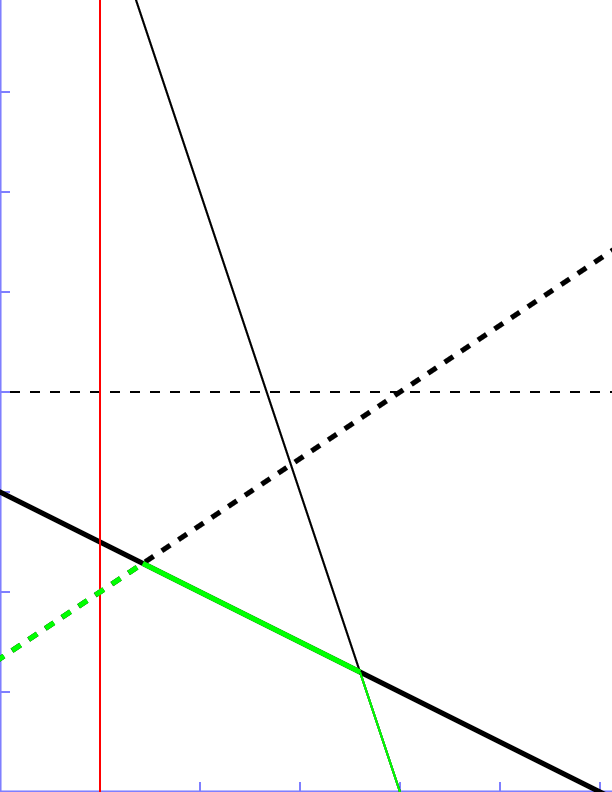
\includegraphics[width=0.5\textwidth]{chtPlot.png} % <- formatos PNG, JPG e PDF
	\label{fig:chtplot}
\end{figure}
\fonte{PEGWIKI, 2016\nocite{Wcipeg2016}}

Para consultar o valor de $x = 1$, que está representado no gráfico acima através da linha vermelha, é possível ver que a reta que gera o menor valor possível é a que está pontilhada com traços grossos, sendo esta a $f(x) = \frac{4}{3} + \frac{2}{3}x$. Analisando esta figura, algumas características importantes podem ser observadas, como é o caso da reta $f(x) = 4$, esta claramente nunca será escolhida, independente do valor de $x$, pois sempre haverá alguma outra que possui um valor menor. Dentre as outras três retas, é possível ver que elas são importantes, pois para algum valor de $x$ elas possuem o menor valor de $f(x)$, isto pode ser visto como a parte em verde pintada nas retas, a qual mostra o intervalo de valores de $x$ onde cada reta é a melhor escolha.
Com a informação de até que ponto uma determinada reta é ótima, elas podem ser ordenadas e cada consulta pode ser resolvida através de uma busca binária\footnote{http://www.geeksforgeeks.org/binary-search/}, onde para cada momento um valor é testado e decidido se a reta ótima para o $x$ em questão está a direita ou a esquerda desta, assim cada consulta teria a complexidade $O(log n)$, sendo $n$ o total de retas.

Uma forma de resolver seria adicionar todas as retas em alguma estrutura de dados, ordená-las pela angulação e depois realizar as consultas. Porém, nem sempre as retas estão disponíveis de antemão, assim, se utilizado a ideia de sempre que adicionar uma nova reta for necessário ordenar todas elas, o algoritmo ficaria com a complexidade $O(n^2*log n)$.
\\

\tikz[baseline=-4pt,align=left]\node[draw,minimum width=12.5cm,minimum height=4ex]
{\textit{Sugere-se ao leitor pensar em uma maneira mais eficaz de adicionar uma nova reta} \\\textit{no conjunto.}};
\\

Partindo do princípio que o conjunto de retas está devidamente ordenado e é necessário inserir mais um reta com angulação maior das já presentes, ao realizar essa operação, alguns casos podem acontecer:
\\
1º) A nova reta não é melhor que nenhuma outra que já estava presente, sendo assim, não há necessidade de incluir esta no conjunto; 
\\
2º) A nova reta é melhor do que algumas outras a partir de algum de valor de $x$;e
\\
3º) A nova reta é melhor que alguma reta em todos os pontos onde esta era ótima, portanto, não é necessário mais manter aquela reta. \\
Com esses casos, um algoritmo mais eficiente pode ser pensado, onde será mantido uma pilha\footnote{http://www.geeksforgeeks.org/stack-data-structure/}, com todas as retas que ainda são ótimas em algum ponto e no seu topo possui a última que foi adicionada. Quando for inserida uma nova reta, basta verificar se a que estava no topo ainda será útil, caso seja, a nova reta é inserida, mas se não for, pode-se realizar um $pop()$ da pilha e ir repetindo este passo até que a pilha esteja vazia, ou que uma reta que ainda é útil for encontrada.

Para determinar o momento que uma reta não é mais relevante e precisa ser removida da pilha, basta verificar se o ponto de intersecção da reta que está sendo inserida no momento com a penúltima reta está a esquerda do ponto de intersecção da penúltima e última reta incluída. Caso isto ocorra, a última reta pode ser removida, pois a partir de agora ela se torna irrelevante. Com essas propriedades é notório que cada reta pode ser adicionada ou removida apenas uma vez, deixando assim a complexidade total $O(n)$ para incluir todas.
\\
Esta técnica possui algumas variações e pode-se destacar três delas:

\textit{\textbf{Convex Hull Trick 1:}}  Nesta versão, as consultas realizadas são feitas de maneira crescente, ou seja, $x_{1}, x_{2}, ..., x_{n}$, portanto, pode ser mantido um ponteiro $p_{i}$, que informa em qual reta estava a resposta para a consulta $x_{i}$, assim quando for necessário descobrir a resposta para a consulta $x_{i+1}$, só é necessário verificar as retas a partir do $p_{i} + 1$. Além disso, todas as retas serão inseridas de maneira ordenada. Isso faz com que todas as consultas sejam respondidas em $O(q + n)$, onde $q$ é o número de consultas e $n$ é o total de retas, isto se deve ao fato de que cada reta será avaliada apenas uma vez, no momento que para alguma consulta esta não for a melhor, é impossível em algum momento ela se tornar ótima.

\textit{\textbf{Convex Hull Trick 2:}} Esta variação é similar com a primeira, porém, as consultas não estão ordenadas, assim, se faz necessário o uso da busca binária, deixando a complexidade em $O(q*log n)$.

\textit{\textbf{Convex Hull Trick 3:}} Nesta versão não há garantias que as retas serão inseridas de forma ordenada, assim, a solução proposta utilizando pilha não funciona mais, portanto, é preciso uma outra estrutura de dados. Com o intuito de deixar a complexidade o mais baixo possível pode ser utilizado uma árvore balanceada para manter as retas ordenadas.
\\

\tikz[baseline=-4pt,align=left]\node[draw,minimum width=12.5cm,minimum height=4ex]
{\textit{Fica como sugestão ao leitor pensar em uma maneira de resolver esta variação.}};
\\


\item \textbf{Benefícios:}
Apesar da técnica demostrada realizar operações em retas, é possível utilizá-la no problema proposto, onde estão são parábolas, mas, como visto na etapa de análise de particularidades, as funções de custo tem a forma $f(x) = ax + b$, ou seja, pode ser descrito da mesma maneira de uma reta, podendo assim ser aplicado neste problema. Como pode ser notado, para resolver o estado $i$, só as retas menores que $i$ são importantes, assim, pode ser inserido a reta relacionado a este estado no momento que ele for resolvido. Devido a solução ingênua elaborada e a ordenação do \textit{array} $v$, é possível ver que as retas inseridas e as consultas realizadas serão feitas de maneira ordenada, portanto pode ser usado a variação 1 do \textit{Convex Hull Trick}. Ao aplicar a otimização, a complexidade será reduzida para $O(n + n) = O(n)$.
\item \textbf{Código final:}
O algoritmo abaixo apresenta a implementação para o problema. Para obter a resposta basta preencher o \textit{array v} com as posições que necessitam de cobertura, este deverá estar com índices entre $1...n$. Ao chamar a função $cht()$, passando como parâmetro a quantidade de elementos e a constante, será devolvido o custo mínimo para realizar a cobertura de todos os pontos.
\\

\tikz[baseline=-4pt,align=left]\node[draw,minimum width=12.5cm,minimum height=4ex]
{\textit{Fica como sugestão ao leitor resolver o problema Covered Walkway} \\\textit{do site Kattis.com}};

\begin{lstlisting}[caption={Implementação Convex Hull Trick 1},label={lst:cht}]
#define MAXN 10
#define inf 99999999
int v[MAXN] = {0, 1, 3, 8, 10};
int dp[MAXN];
int A[MAXN], B[MAXN];
int tam, ponteiro;

int quadrado(int x){ return x*x; }

void adicionarLinha(int a, int b){
	while(tam >= 2 && 
			(B[tam-2] - B[tam-1]) * (a-A[tam-1]) >=
			 (B[tam-1]-b) * (A[tam-1]-A[tam-2]))
		tam--;
	A[tam] = a;
	B[tam] = b;
	tam++;
}

int consultar(int x){
	ponteiro = min(ponteiro, tam-1);
	while(ponteiro+1 < tam && 
		A[ponteiro+1]*x+B[ponteiro+1] <= A[ponteiro]*x + B[ponteiro])
		ponteiro++;
	return A[ponteiro]*x + B[ponteiro];
}

int cht(int n, int c){
	// Inicializando a pilha do Convex Hull Trick
	ponteiro = tam = 0;
	
	// Caso base
	dp[0] = 0;
	adicionarLinha(-2*v[1], quadrado(v[1]));
	for(int i = 1; i <= n; i++){
		dp[i] = consultar(v[i]) + quadrado(v[i]) + c;
		if(i < n)
			adicionarLinha(-2*v[i+1], quadrado(v[i+1])+dp[i]);
	}
	return dp[n];
}


\end{lstlisting}
\end{itemize}

